% questions.tex —— 2016 年·全国Ⅰ卷·理科 · 题目内容片段（无答案）
% 由 tools/generate_projects.py 依来源总账自 2016/2016_数学真题_全国1理_试题.md 生成，勿手改（改源 MD 后重跑）


\gkpart{数学}

\begin{gktip}
\textbf{来源说明}：本题面依据固定源 PDF 两页 A3 页面逐题核对，原卷印刷页码 999–1000。固定源不附答案；本文件仅为题面规范源。
\end{gktip}

\gkpart{一、选择题}

\begin{question}
\gkti{1}设集合 $A=\{x\mid x^2-4x+3<0\}$，$B=\{x\mid 2x-3>0\}$，则 $A\cap B=$（　）

   (A) $(-3,-\frac32)$　(B) $(-3,\frac32)$　(C) $(1,\frac32)$　(D) $(\frac32,3)$

\end{question}
\begin{question}
\gkti{2}设 $(1+i)x=1+yi$，其中 $x,y$ 是实数，则 $|x+yi|=$（　）

   (A) $1$　(B) $\sqrt2$　(C) $\sqrt3$　(D) $2$

\end{question}
\begin{question}
\gkti{3}已知等差数列 $\{a_n\}$ 前 $9$ 项的和为 $27$，$a_{10}=8$，则 $a_{100}=$（　）

   (A) $100$　(B) $99$　(C) $98$　(D) $97$

\end{question}
\begin{question}
\gkti{4}某公司的班车在 $7{:}30$，$8{:}00$，$8{:}30$ 发车，小明在 $7{:}50$ 至 $8{:}30$ 之间到达发车站乘坐班车，且到达发车站的时刻是随机的，则他等车时间不超过 $10$ 分钟的概率是（　）

   (A) $\frac13$　(B) $\frac12$　(C) $\frac23$　(D) $\frac34$

\end{question}
\begin{question}
\gkti{5}已知方程 $\dfrac{x^2}{m^2+n}-\dfrac{y^2}{3m^2-n}=1$ 表示双曲线，且该双曲线两焦点间的距离为 $4$，则 $n$ 的取值范围是（　）

   (A) $(-1,3)$　(B) $(-1,\sqrt3)$　(C) $(0,3)$　(D) $(0,\sqrt3)$

\Needspace{0.4\textheight}
\end{question}
\begin{question}
\gkti{6}如图，某几何体的三视图是三个半径相等的圆及每个圆中两条相互垂直的半径。若该几何体的体积是 $\dfrac{28\pi}{3}$，则它的表面积是（　）

   (A) $17\pi$　(B) $18\pi$　(C) $20\pi$　(D) $28\pi$
\nopagebreak[4]
\begin{center}% 2016 全国卷Ⅰ理科第 6 题：三个圆形投影及各自的两条垂直半径。
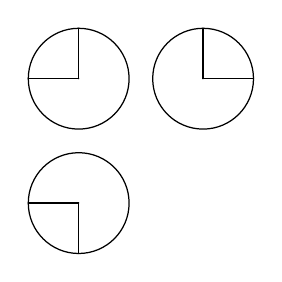
\begin{tikzpicture}[line width=.45pt,line cap=round,line join=round]
  \coordinate (upperleft) at (0,0);
  \coordinate (upperright) at (1.58,0);
  \coordinate (lowerleft) at (0,-1.58);
  \def\r{.64}
  \draw (upperleft) circle[radius=\r];
  \draw (upperright) circle[radius=\r];
  \draw (lowerleft) circle[radius=\r];
  \draw (upperleft) -- (0,\r) (-\r,0) -- (upperleft);
  \draw (upperright) -- (1.58,\r) (upperright) -- (1.58+\r,0);
  \draw (lowerleft) -- (-\r,-1.58) (lowerleft) -- (0,-1.58-\r);
\end{tikzpicture}
\end{center}
\nopagebreak[4]
\Needspace{0.4\textheight}
\end{question}
\begin{question}
\gkti{7}函数 $y=2x^2-e^{|x|}$ 在 $[-2,2]$ 的图象大致为（　）
\nopagebreak[4]
\begin{center}% 2016 全国卷Ⅰ理科第 7 题：函数图象选择项 A–D。
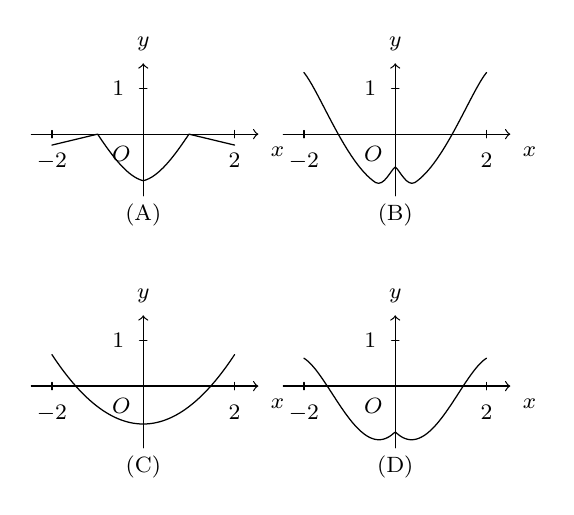
\begin{tikzpicture}[x=.58cm,y=.58cm,font=\footnotesize,line width=.45pt,
  line cap=round,line join=round]
  % A：两侧在 x 轴下方，曲线在 x=±1 处到达尖点。
  \begin{scope}[yshift=3.2cm]
    \draw[->] (-2.45,0) -- (2.52,0);
    \draw[->] (0,-1.35) -- (0,1.55);
    \draw (-2,.08)--(-2,-.08) node[below=2pt] {$-2$};
    \draw (2,.08)--(2,-.08) node[below=2pt] {$2$};
    \draw (.08,1)--(-.08,1) node[left=2pt] {$1$};
    \node[below left=1pt] at (0,0) {$O$};
    \node[below right=1pt] at (2.52,0) {$x$};
    \node[above=1pt] at (0,1.55) {$y$};
    \draw (-2,-.24) -- (-1,0)
      .. controls (-.68,-.48) and (-.34,-.94) .. (0,-1.02)
      .. controls (.34,-.94) and (.68,-.48) .. (1,0)
      -- (2,-.24);
    \node at (0,-1.76) {(A)};
  \end{scope}

  % B：两端高于 y=1，中央为带尖顶的双谷。
  \begin{scope}[xshift=3.2cm,yshift=3.2cm]
    \draw[->] (-2.45,0) -- (2.52,0);
    \draw[->] (0,-1.35) -- (0,1.55);
    \draw (-2,.08)--(-2,-.08) node[below=2pt] {$-2$};
    \draw (2,.08)--(2,-.08) node[below=2pt] {$2$};
    \draw (.08,1)--(-.08,1) node[left=2pt] {$1$};
    \node[below left=1pt] at (0,0) {$O$};
    \node[below right=1pt] at (2.52,0) {$x$};
    \node[above=1pt] at (0,1.55) {$y$};
    \draw (-2,1.35)
      .. controls (-1.65,.92) and (-1.08,-.63) .. (-.43,-1.06)
      .. controls (-.25,-1.16) and (-.10,-.79) .. (0,-.72)
      .. controls (.10,-.79) and (.25,-1.16) .. (.43,-1.06)
      .. controls (1.08,-.63) and (1.65,.92) .. (2,1.35);
    \node at (0,-1.76) {(B)};
  \end{scope}

  % C：两端高于 x 轴，中央为平滑单谷。
  \begin{scope}
    \draw[->] (-2.45,0) -- (2.52,0);
    \draw[->] (0,-1.35) -- (0,1.55);
    \draw (-2,.08)--(-2,-.08) node[below=2pt] {$-2$};
    \draw (2,.08)--(2,-.08) node[below=2pt] {$2$};
    \draw (.08,1)--(-.08,1) node[left=2pt] {$1$};
    \node[below left=1pt] at (0,0) {$O$};
    \node[below right=1pt] at (2.52,0) {$x$};
    \node[above=1pt] at (0,1.55) {$y$};
    \draw[domain=-2:2,samples=80,variable=\x]
      plot ({\x},{.38*\x*\x-.83});
    \node at (0,-1.76) {(C)};
  \end{scope}

  % D：按题给函数绘出对称双谷，端点位于 x 轴上方、y=1 下方。
  \begin{scope}[xshift=3.2cm]
    \draw[->] (-2.45,0) -- (2.52,0);
    \draw[->] (0,-1.35) -- (0,1.55);
    \draw (-2,.08)--(-2,-.08) node[below=2pt] {$-2$};
    \draw (2,.08)--(2,-.08) node[below=2pt] {$2$};
    \draw (.08,1)--(-.08,1) node[left=2pt] {$1$};
    \node[below left=1pt] at (0,0) {$O$};
    \node[below right=1pt] at (2.52,0) {$x$};
    \node[above=1pt] at (0,1.55) {$y$};
    \draw[domain=-2:2,samples=120,variable=\x]
      plot ({\x},{2*\x*\x-exp(abs(\x))});
    \node at (0,-1.76) {(D)};
  \end{scope}
\end{tikzpicture}
\end{center}
\nopagebreak[4]
\end{question}
\begin{question}
\gkti{8}若 $a>b>1$，$0<c<1$，则（　）

   (A) $a^c<b^c$　(B) $ab^c<ba^c$

   (C) $a\log_b c<b\log_a c$　(D) $\log_a c<\log_b c$

\Needspace{0.4\textheight}
\end{question}
\begin{question}
\gkti{9}执行下面的程序框图，如果输入的 $x=0$，$y=1$，$n=1$，则输出 $x,y$ 的值满足（　）
\nopagebreak[4]
\begin{center}% 2016 全国卷Ⅰ理科第 9 题：循环程序框图。
\begin{tikzpicture}[font=\footnotesize,>=Stealth,line width=.4pt,
  line cap=round,line join=round,
  term/.style={draw,rounded corners=5pt,minimum height=1.55em,minimum width=1.3em,inner xsep=6pt},
  io/.style={draw,trapezium,trapezium left angle=70,trapezium right angle=110,
    minimum height=1.65em,minimum width=2.2cm,inner xsep=5pt},
  box/.style={draw,minimum height=1.65em,inner xsep=5pt},
  dec/.style={draw,diamond,aspect=3.0,minimum width=3.6cm,inner sep=1.5pt}]
  \node[term] (start) at (0,0) {开始};
  \node[io] (input) at (0,-.85) {输入 $x,y,n$};
  \node[box,minimum width=4.6cm] (calc) at (0,-1.95)
    {$\displaystyle x=x+\frac{n-1}{2},\ y=ny$};
  \node[dec] (cond) at (0,-3.5) {$x^2+y^2\geqslant36$};
  \node[box,minimum width=1.55cm] (inc) at (-2.8,-2.9) {$n=n+1$};
  \node[io] (output) at (0,-4.95) {输出 $x,y$};
  \node[term] (end) at (0,-5.85) {结束};

  \draw[->] (start) -- (input);
  \draw[->] (input.south) -- (calc.north);
  \draw[->] (calc) -- (cond);
  \draw[->] (cond.south) -- node[right,pos=.48] {是} (output.north);
  \draw[->] (output) -- (end);

  \coordinate (no) at ([xshift=-6mm]cond.west);
  \node[below=1pt] at (no) {否};
  \draw[->] (cond.west) -- (no) -| (inc.south);

  \coordinate (returnEntry) at ([xshift=-14mm]calc.north);
  \draw[->] (inc.north) -- ++(0,1.45) -| (returnEntry);
\end{tikzpicture}
\end{center}
\nopagebreak[4]
   (A) $y=2x$　(B) $y=3x$　(C) $y=4x$　(D) $y=5x$

\end{question}
\begin{question}
\gkti{10}以抛物线 $C$ 的顶点为圆心的圆交 $C$ 于 $A,B$ 两点，交 $C$ 的准线于 $D,E$ 两点。已知 $|AB|=4\sqrt2$，$|DE|=2\sqrt5$，则 $C$ 的焦点到准线的距离为（　）

   (A) $2$　(B) $4$　(C) $6$　(D) $8$

\end{question}
\begin{question}
\gkti{11}平面 $\alpha$ 过正方体 $ABCD-A_1B_1C_1D_1$ 的顶点 $A$，$\alpha\parallel$ 平面 $CB_1D_1$，$\alpha\cap$ 平面 $ABCD=m$，$\alpha\cap$ 平面 $ABB_1A_1=n$，则 $m,n$ 所成角的正弦值为（　）

   (A) $\frac{\sqrt3}{2}$　(B) $\frac{\sqrt2}{2}$　(C) $\frac{\sqrt3}{3}$　(D) $\frac13$

\end{question}
\begin{question}
\gkti{12}已知函数 $f(x)=\sin(\omega x+\varphi)$（$\omega>0$，$|\varphi|\leq\frac\pi2$），$x=-\frac\pi4$ 为 $f(x)$ 的零点，$x=\frac\pi4$ 为 $y=f(x)$ 图象的对称轴，且 $f(x)$ 在 $(\frac\pi{18},\frac{5\pi}{36})$ 单调，则 $\omega$ 的最大值为（　）

   (A) $11$　(B) $9$　(C) $7$　(D) $5$

\end{question}
\gkpart{二、填空题}

\begin{question}
\gkti{13}设向量 $\boldsymbol a=(m,1)$，$\boldsymbol b=(1,2)$，且 $|\boldsymbol a+\boldsymbol b|^2=|\boldsymbol a|^2+|\boldsymbol b|^2$，则 $m=$\gkblank{}。

\end{question}
\begin{question}
\gkti{14}$(2x+\sqrt{x})^5$ 的展开式中，$x^3$ 的系数是\gkblank{}。（用数字填写答案）

\end{question}
\begin{question}
\gkti{15}设等比数列满足 $a_1+a_3=10$，$a_2+a_4=5$，则 $a_1a_2\cdots a_n$ 的最大值为\gkblank{}。

\end{question}
\begin{question}
\gkti{16}某高科技企业生产产品 $A$ 和产品 $B$，需要甲、乙两种新型材料。生产一件产品 $A$ 需要甲材料 $1.5\,\mathrm{kg}$、乙材料 $1\,\mathrm{kg}$，用 $5$ 个工时；生产一件产品 $B$ 需要甲材料 $0.5\,\mathrm{kg}$、乙材料 $0.3\,\mathrm{kg}$，用 $3$ 个工时。生产一件产品 $A$ 的利润为 $2100$ 元，生产一件产品 $B$ 的利润为 $900$ 元。该企业现有甲材料 $150\,\mathrm{kg}$、乙材料 $90\,\mathrm{kg}$，则在不超过 $600$ 个工时的条件下，生产产品 $A$、产品 $B$ 的利润之和的最大值为\gkblank{}元。

\end{question}
\gkpart{三、解答题}

\begin{question}
\gkti{17}$\triangle ABC$ 的内角 $A,B,C$ 的对边分别为 $a,b,c$，已知 $2\cos C(a\cos B+b\cos A)=c$。

   (1) 求 $C$；

   (2) 若 $c=\sqrt7$，$\triangle ABC$ 的面积为 $\dfrac{3\sqrt3}{2}$，求 $\triangle ABC$ 的周长。

\Needspace{0.4\textheight}
\end{question}
\begin{question}
\gkti{18}如图，在以 $A,B,C,D,E,F$ 为顶点的五面体中，面 $ABEF$ 为正方形，$AF=2FD$，$\angle AFD=90^\circ$，且二面角 $D-AF-E$ 与二面角 $C-BE-F$ 都是 $60^\circ$。
\nopagebreak[4]
\begin{center}% 2016 全国卷Ⅰ理科第 18 题：五面体的可见棱；交叉处不是顶点。
\begin{tikzpicture}[font=\footnotesize,line width=.45pt,line cap=round,line join=round]
  \coordinate (F) at (0,0);
  \coordinate (D) at (1.55,2.25);
  \coordinate (A) at (2.60,-1.25);
  \coordinate (C) at (4.15,2.55);
  \coordinate (E) at (4.90,.45);
  \coordinate (B) at (7.50,-.35);

  % 原图中的三条虚棱；F--E 与实棱 D--A 相交但不构成顶点。
  \draw[dashed] (F)--(E) (E)--(C) (E)--(B);
  % 原图中的可见实棱。
  \draw (D)--(C) (C)--(B) (B)--(A) (A)--(F) (F)--(D) (D)--(A);

  \node[left] at (F) {$F$};
  \node[above left] at (D) {$D$};
  \node[above] at (C) {$C$};
  \node[right] at (E) {$E$};
  \node[below] at (A) {$A$};
  \node[below right] at (B) {$B$};
\end{tikzpicture}
\end{center}
\nopagebreak[4]
   (1) 证明：平面 $ABEF\perp$ 平面 $EFDC$；

   (2) 求二面角 $E-BC-A$ 的余弦值。

\Needspace{0.4\textheight}
\end{question}
\begin{question}
\gkti{19}某公司计划购买 $2$ 台机器，该种机器使用三年后即被淘汰。机器有一易损零件，在购进机器时，可以额外购买这种零件作为备件，每个 $200$ 元。在机器使用期间，如果备件不足再购买，则每个 $500$ 元。现需决策在购买机器时应同时购买几个易损零件，为此搜集并整理了 $100$ 台这种机器在三年使用期内更换的易损零件数，得下面柱状图：
\nopagebreak[4]
\begin{center}% 2016 全国卷Ⅰ理科第 19 题：易损零件更换数的频数柱状图。
\begin{tikzpicture}[x=.46cm,y=.055cm,font=\footnotesize,line width=.4pt,
  line cap=round,line join=round]
  % 频数 20、40 的水平参考虚线。
  \draw[dashed] (0,20)--(11.35,20);
  \draw[dashed] (0,40)--(9.00,40);

  % 四个柱：8、9、10、11 对应频数 20、40、20、20。
  \draw (7.67,0) rectangle (8.33,20);
  \draw (8.67,0) rectangle (9.33,40);
  \draw (9.67,0) rectangle (10.33,20);
  \draw (10.67,0) rectangle (11.33,20);

  % 纵轴及原点附近的横轴断轴记号。
  \draw (0,0)--(0,44);
  \draw[->] (0,44)--(0,47);
  \draw (0,0)--(.28,0);
  \draw (.28,0)--(.38,2.2)--(.52,-2.2)--(.66,2.2)--(.80,0);
  \draw[->] (.80,0)--(12.15,0);

  \node[left=2pt] at (0,20) {20};
  \node[left=2pt] at (0,40) {40};
  \node[below left=1pt] at (0,0) {0};
  \node[above right=1pt] at (0,47) {频数};
  \node[below] at (8,0) {8};
  \node[below] at (9,0) {9};
  \node[below] at (10,0) {10};
  \node[below] at (11,0) {11};
  \node[anchor=west] at (12.35,0) {更换的易损零件数};
\end{tikzpicture}
\end{center}
\nopagebreak[4]
   以这 $100$ 台机器更换的易损零件数的频率代替 $1$ 台机器更换的易损零件数发生的概率，记 $X$ 表示 $2$ 台机器三年内共需更换的易损零件数，$n$ 表示购买 $2$ 台机器的同时购买的易损零件数。

   (1) 求 $X$ 的分布列；

   (2) 若要求 $P(X\leq n)\geq0.5$，确定 $n$ 的最小值；

   (3) 以购买易损零件所需费用的期望值为决策依据，在 $n=19$ 与 $n=20$ 之中选其一，应选用哪个？

\end{question}
\begin{question}
\gkti{20}设圆 $x^2+y^2+2x-15=0$ 的圆心为 $A$，直线 $l$ 过点 $B(1,0)$ 且与 $x$ 轴不重合，$l$ 交圆 $A$ 于 $C,D$ 两点，过 $B$ 作 $AC$ 的平行线交 $AD$ 于点 $E$。

   (1) 证明 $|EA|+|EB|$ 为定值，并写出点 $E$ 的轨迹方程；

   (2) 设点 $E$ 的轨迹为曲线 $C_1$，直线 $l$ 交 $C_1$ 于 $M,N$ 两点，过 $B$ 且与 $l$ 垂直的直线与圆 $A$ 交于 $P,Q$ 两点，求四边形 $MPNQ$ 面积的取值范围。

\end{question}
\begin{question}
\gkti{21}已知函数 $f(x)=(x-2)e^x+a(x-1)^2$ 有两个零点。

   (1) 求 $a$ 的取值范围；

   (2) 设 $x_1,x_2$ 是 $f(x)$ 的两个零点，证明：$x_1+x_2<2$。

\Needspace{0.4\textheight}
\end{question}
\begin{question}
\gkti{22}如图，$\triangle OAB$ 是等腰三角形，$\angle AOB=120^\circ$，以 $O$ 为圆心，$\frac12 OA$ 为半径作圆。
\nopagebreak[4]
\begin{center}% 2016 全国卷Ⅰ理科第 22 题：圆、弦 CD 与相切的等腰三角形 OAB。
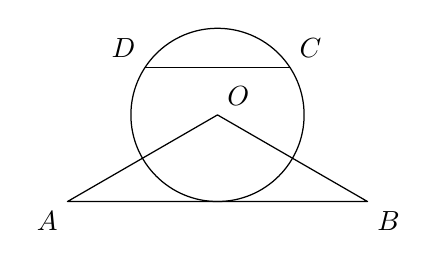
\begin{tikzpicture}[line width=.45pt,line cap=round,line join=round]
  \coordinate (O) at (0,0);
  \coordinate (A) at (-1.905,-1.10);
  \coordinate (B) at (1.905,-1.10);
  \coordinate (D) at (-.919,.605);
  \coordinate (C) at (.919,.605);

  \draw (O) circle[radius=1.10];
  \draw (D)--(C);
  \draw (O)--(A) (O)--(B) (A)--(B);

  \node[above right] at (O) {$O$};
  \node[above left] at (D) {$D$};
  \node[above right] at (C) {$C$};
  \node[below left] at (A) {$A$};
  \node[below right] at (B) {$B$};
\end{tikzpicture}
\end{center}
\nopagebreak[4]
   (1) 证明：直线 $AB$ 与 $\odot O$ 相切；

   (2) 点 $C,D$ 在 $\odot O$ 上，且 $A,B,C,D$ 四点共圆，证明：$AB\parallel CD$。

\end{question}
\begin{question}
\gkti{23}在直角坐标系 $xOy$ 中，曲线 $C_1$ 的参数方程为
\nopagebreak[4]
   \[
   \begin{cases}
   x=a\cos t,\\
   y=1+a\sin t,
   \end{cases}\qquad (t\text{ 为参数},\ a>0).
   \]
   在以坐标原点为极点，$x$ 轴正半轴为极轴的极坐标系中，曲线 $C_2$：$\rho=4\cos\theta$。

   (1) 说明 $C_1$ 是哪种曲线，并将 $C_1$ 的方程化为极坐标方程；

   (2) 直线 $C_3$ 的极坐标方程为 $\theta=\alpha_0$，其中 $\alpha_0$ 满足 $\tan\alpha_0=2$。若曲线 $C_1$ 与 $C_2$ 的公共点都在 $C_3$ 上，求 $a$。

\Needspace{0.4\textheight}
\end{question}
\begin{question}
\gkti{24}已知函数 $f(x)=|x+1|-|2x-3|$。

   (1) 在图中画出 $y=f(x)$ 的图象；

   (2) 求不等式 $|f(x)|>1$ 的解集。
\nopagebreak[4]
\begin{center}% 2016 全国卷Ⅰ理科第 24 题：作图用直角坐标网格。
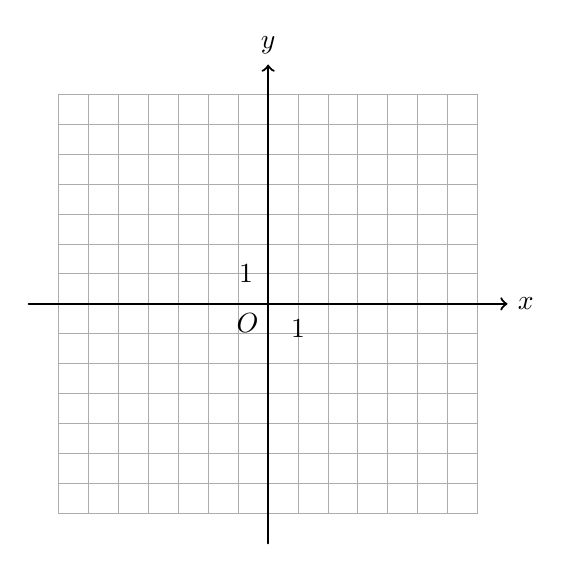
\begin{tikzpicture}[x=0.38cm,y=0.38cm,line cap=round,line join=round]
\foreach \x in {-7,-6,...,7} {
  \draw[gray!65,line width=0.35pt] (\x,-7) -- (\x,7);
}
\foreach \y in {-7,-6,...,7} {
  \draw[gray!65,line width=0.35pt] (-7,\y) -- (7,\y);
}
\draw[->,thick] (-8,0) -- (8,0) node[right] {$x$};
\draw[->,thick] (0,-8) -- (0,8) node[above] {$y$};
\node[below left] at (0,0) {$O$};
\node[left=2pt] at (0,1) {$1$};
\node[below=2pt] at (1,0) {$1$};
\end{tikzpicture}
\end{center}
\nopagebreak[4]

\end{question}